\documentclass[a4paper,10pt,titlepage]{report}
%%This template is based on Paco van Beckhoven's thesis. 

\usepackage{xspace}
\usepackage{xargs}   % Use more than one optional parameter in a new commands
\usepackage[pdftex,dvipsnames]{xcolor}

% Putting images next to each other
\usepackage[font=bf,]{caption}
\usepackage{subcaption}
\input{glyphtounicode}

% for last page
\usepackage{lastpage}

\usepackage[english]{babel}
\usepackage[utf8]{inputenc}
\usepackage{csquotes}
\usepackage[margin=1in]{geometry}
\usepackage{fancyhdr}
\usepackage{booktabs}
\usepackage{paralist}
\usepackage{graphicx}
\usepackage{tabularx}
\usepackage{adjustbox}
\usepackage{titlepic}
\usepackage{vhistory}
\usepackage{enumitem}
\usepackage{longtable}
\usepackage[backend=biber, style=ieee,citestyle=numeric-comp]{biblatex}
\usepackage[colorinlistoftodos, prependcaption]{todonotes}
\usepackage{placeins}
\usepackage{multirow}
\usepackage{amsmath,amssymb}
\usepackage[hidelinks]{hyperref}
\usepackage[acronym,nogroupskip,nohypertypes={acronym},toc,section=chapter]{glossaries}
\usepackage{amssymb}
\usepackage{verbatim}
\usepackage{cmap}
\usepackage{subfiles}
\usepackage{dirtytalk}

%\usepackage[ansinew]{inputenc}
%\usepackage[T1]{fontenc}
%\usepackage{libertine}
\input{glyphtounicode}

\pdfglyphtounicode{f_f}{FB00}
\pdfglyphtounicode{f_f_i}{FB03}
\pdfglyphtounicode{f_f_l}{FB04}
\pdfglyphtounicode{f_i}{FB01}

\pdfgentounicode=1



%Appendix package + appendix in chapter title
\usepackage[titletoc]{appendix}




%for highlighting findings
\usepackage{tcolorbox}

% for highlighting code examples
\usepackage{listings}
\usepackage{uvaTemplate}

%helpful acronym examples
\newacronym{poc}{POC}{proof-of-concept}

\newacronym{sut}{SUT}{System Under Test}

\newacronym{tloc}{TLOC}{Lines Of Test Code}

\newacronym{loc}{LOC}{Lines of Code}

\newacronym{cli}{CLI}{Command Line Interface}

\newacronym{csv}{CSV}{comma-separated values}

\newacronym{som}{SOM}{self organizing map}

\newacronym{fcm}{FCM}{fuzzy c-means}

\newacronym{lvq}{LVQ}{learning vector quantization}

\makeglossaries
\bibliography{main}
\bibliography{custom}

\begin{document}

\title{Mutation testing: clustering mutants}
\author{Rasjaad Basarat}
\authoremail{rasjaad.basarat@student.uva.nl}
\academicsupervisor{Ana Oprescu}
\academicsupervisoremail{a.m.oprescu@uva.nl}
\dailysupervisor{Thomas Biesaart}
\dailysupervisoremail{thomas@infi.nl}
\hostorg{Infi}
\hostorgurl{https://infi.nl}
\maketitle

\subfile{chapters/1_abstract}

\tableofcontents

\subfile{chapters/2_introduction}
\subfile{chapters/3_background}
\subfile{chapters/4_mutation_tool}
\subfile{chapters/5_identifying_characteristics}
\subfile{chapters/6_experiment_design}
\subfile{chapters/99_research}
\subfile{chapters/results}
\subfile{chapters/discussion}
\subfile{chapters/related_work}
\subfile{chapters/conclusion}
\subfile{chapters/acknowledgements}

\printbibliography[heading=bibintoc]
\printglossaries%

\begin{appendices}
	
\chapter{PIT maven code}
\label{ap:PIT_maven_code}
Example of code used to execute a full set of mutants with PIT.
\begin{lstlisting}
    <plugins>
      <plugin>
        <groupId>org.pitest</groupId>
        <artifactId>pitest-maven</artifactId>
        <version>1.6.4</version>
        <dependencies>
          <dependency>
            <groupId>com.niverhawk</groupId>
            <artifactId>pitest-clustering-plugin</artifactId>
            <version>1.0-SNAPSHOT</version>
          </dependency>
        </dependencies>
        <configuration>
          <exportLineCoverage>true</exportLineCoverage>
          <mutators>
            <mutator>ALL</mutator>
          </mutators>
          <threads>6</threads>
        </configuration>
      </plugin>
\end{lstlisting}

\chapter{Box-plots of samples per project with all characteristics n*0.25 reduction}
\label{ap:full_25}
\begin{figure}[h]
    \centering
    \subfloat{{\includegraphics[scale=0.32]{images/full_25/boxplot_google-auto-service.png}}}
    \qquad
    \subfloat{{\includegraphics[scale=0.32]{images/full_25/boxplot_scribejava-core.png}}}
\end{figure}

\begin{figure}[h]
    \centering
    \subfloat{{\includegraphics[scale=0.3]{images/full_25/boxplot_google-auto-factory.png}}}
    \qquad
    \subfloat{{\includegraphics[scale=0.3]{images/full_25/boxplot_google-auto-common.png}}}
\end{figure}

\begin{figure}[h]
    \centering
    \subfloat{{\includegraphics[scale=0.3]{images/full_25/boxplot_google-auto-value.png}}}
    \qquad
    \subfloat{{\includegraphics[scale=0.3]{images/full_25/boxplot_gson.png}}}
\end{figure}

\begin{figure}[h]
    \centering
    \subfloat{{\includegraphics[scale=0.3]{images/full_25/boxplot_commons-io.png}}}
    \qquad
    \subfloat{{\includegraphics[scale=0.3]{images/full_25/boxplot_commons-cli.png}}}
\end{figure}

\begin{figure}[h]
    \centering
    \subfloat{{\includegraphics[scale=0.3]{images/full_25/boxplot_commons-text.png}}}
    \qquad
    \subfloat{{\includegraphics[scale=0.3]{images/full_25/boxplot_commonc-codec.png}}}
\end{figure}

\begin{figure}[h]
\centering
\includegraphics[scale=0.3]{images/full_25/boxplot_commons-csv.png}
\end{figure}

\chapter{Box-plots of samples per project with all characteristics n*0.50 reduction}
\label{ap:full_50}
\begin{figure}[h]
    \centering
    \subfloat{{\includegraphics[scale=0.32]{images/full_50/boxplot_google-auto-service.png}}}
    \qquad
    \subfloat{{\includegraphics[scale=0.32]{images/full_50/boxplot_scribejava-core.png}}}
\end{figure}

\begin{figure}[h]
    \centering
    \subfloat{{\includegraphics[scale=0.3]{images/full_50/boxplot_google-auto-factory.png}}}
    \qquad
    \subfloat{{\includegraphics[scale=0.3]{images/full_50/boxplot_google-auto-common.png}}}
\end{figure}

\begin{figure}[h]
    \centering
    \subfloat{{\includegraphics[scale=0.3]{images/full_50/boxplot_google-auto-value.png}}}
    \qquad
    \subfloat{{\includegraphics[scale=0.3]{images/full_50/boxplot_gson.png}}}
\end{figure}

\begin{figure}[h]
    \centering
    \subfloat{{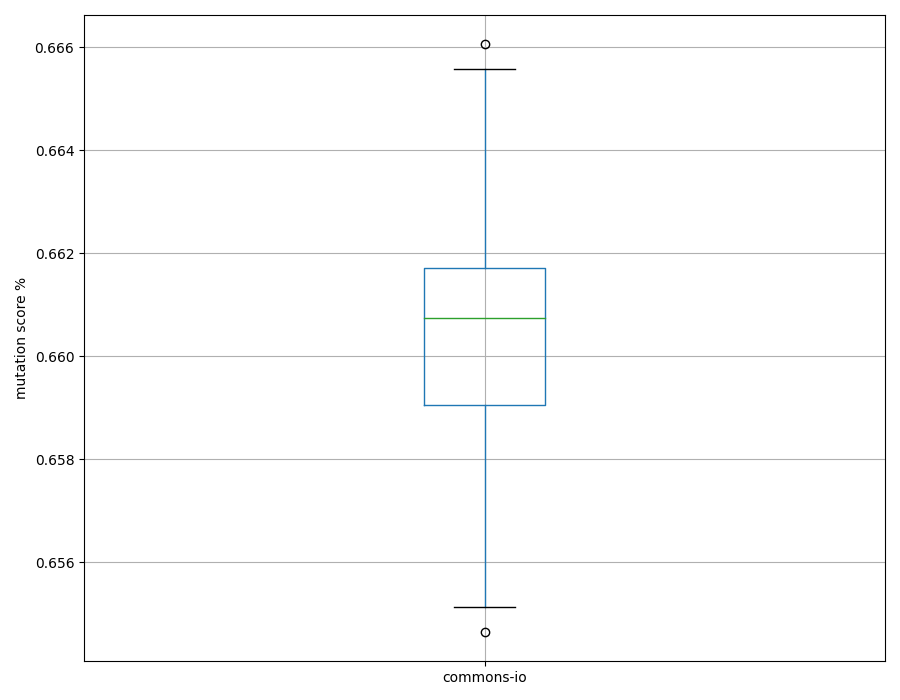
\includegraphics[scale=0.3]{images/full_50/boxplot_commons-io.png}}}
    \qquad
    \subfloat{{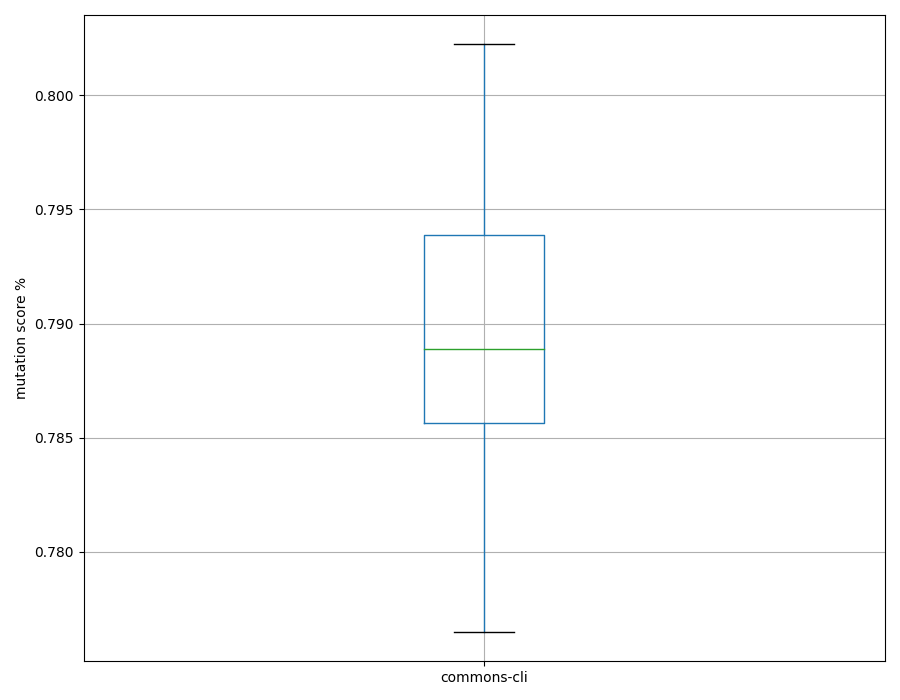
\includegraphics[scale=0.3]{images/full_50/boxplot_commons-cli.png}}}
\end{figure}

\begin{figure}[h]
    \centering
    \subfloat{{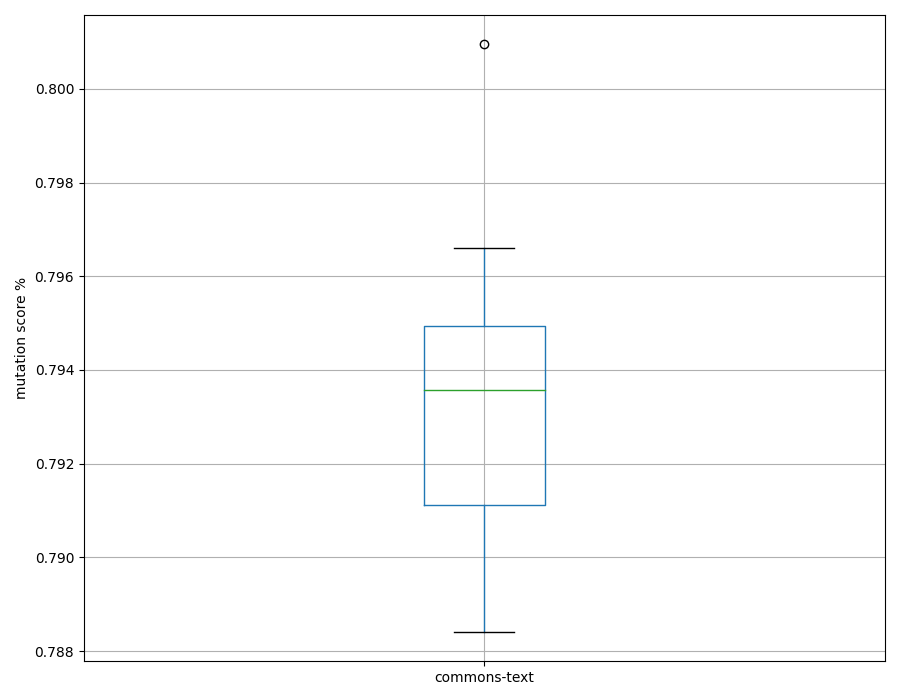
\includegraphics[scale=0.3]{images/full_50/boxplot_commons-text.png}}}
    \qquad
    \subfloat{{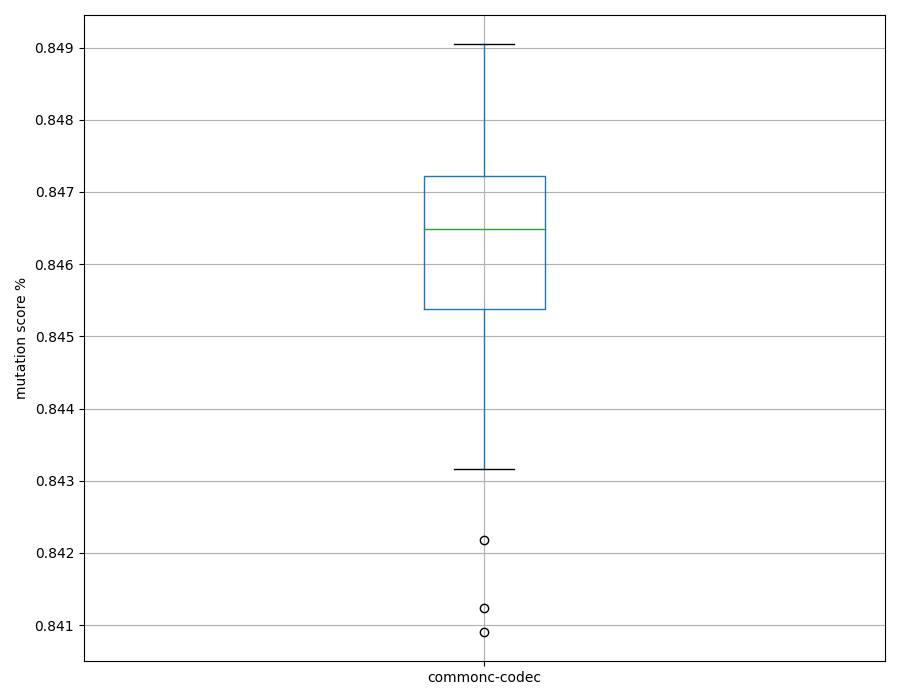
\includegraphics[scale=0.3]{images/full_50/boxplot_commonc-codec.png}}}
\end{figure}

\begin{figure}[h]
\centering
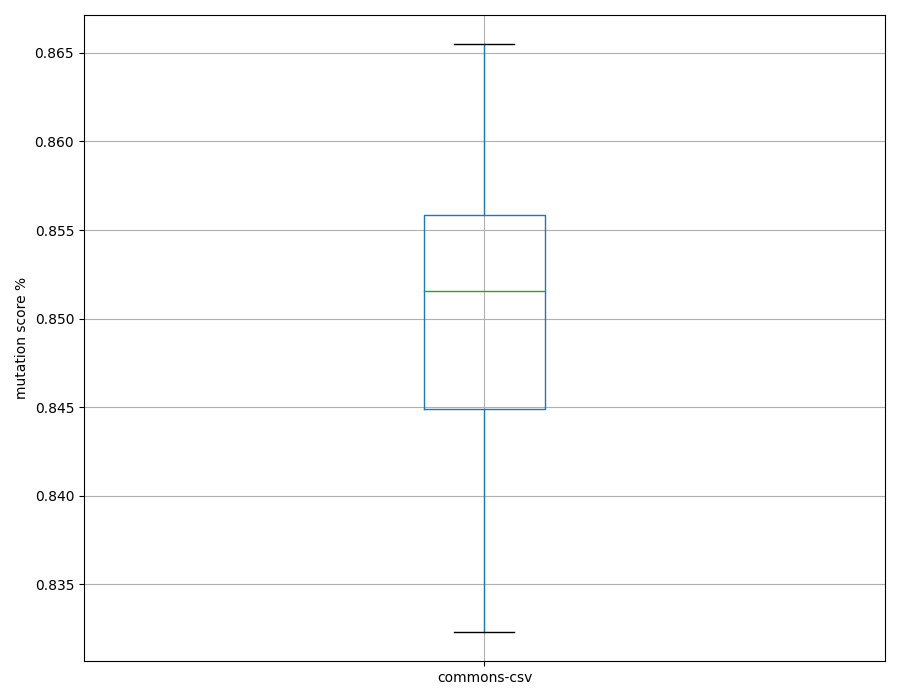
\includegraphics[scale=0.3]{images/full_50/boxplot_commons-csv.png}
\end{figure}

\chapter{Box-plots of samples per project with all characteristics n*0.75 reduction}
\label{ap:full_75}
\begin{figure}[h]
    \centering
    \subfloat{{\includegraphics[scale=0.32]{images/full_75/boxplot_google-auto-service.png}}}
    \qquad
    \subfloat{{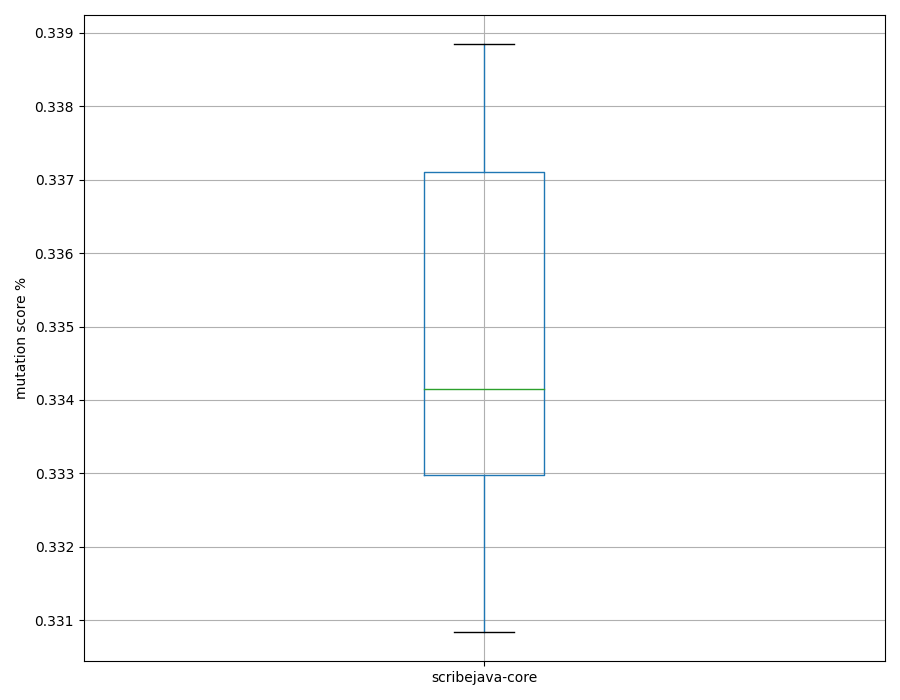
\includegraphics[scale=0.32]{images/full_75/boxplot_scribejava-core.png}}}
\end{figure}

\begin{figure}[h]
    \centering
    \subfloat{{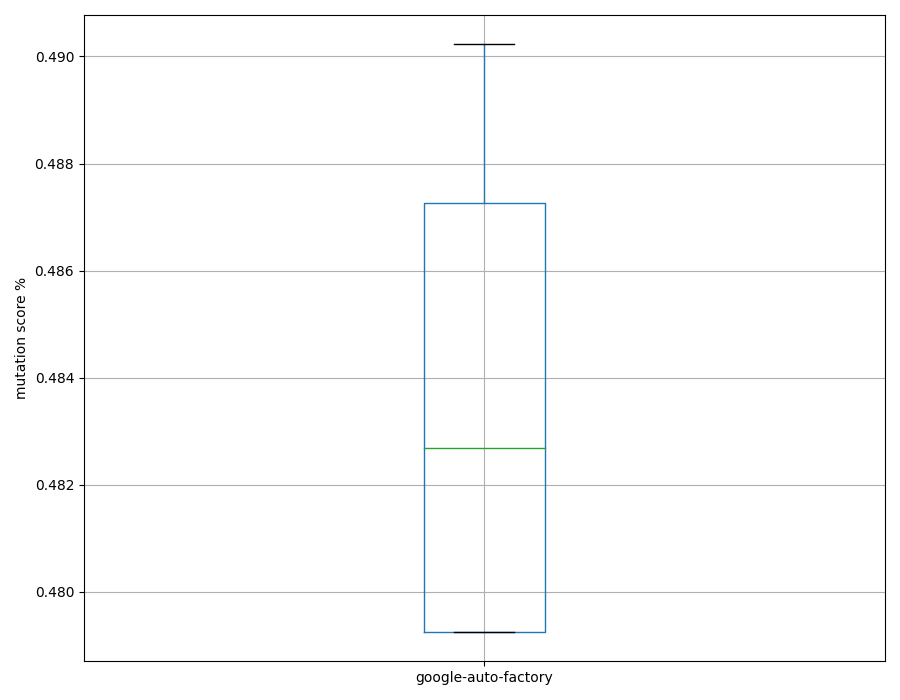
\includegraphics[scale=0.3]{images/full_75/boxplot_google-auto-factory.png}}}
    \qquad
    \subfloat{{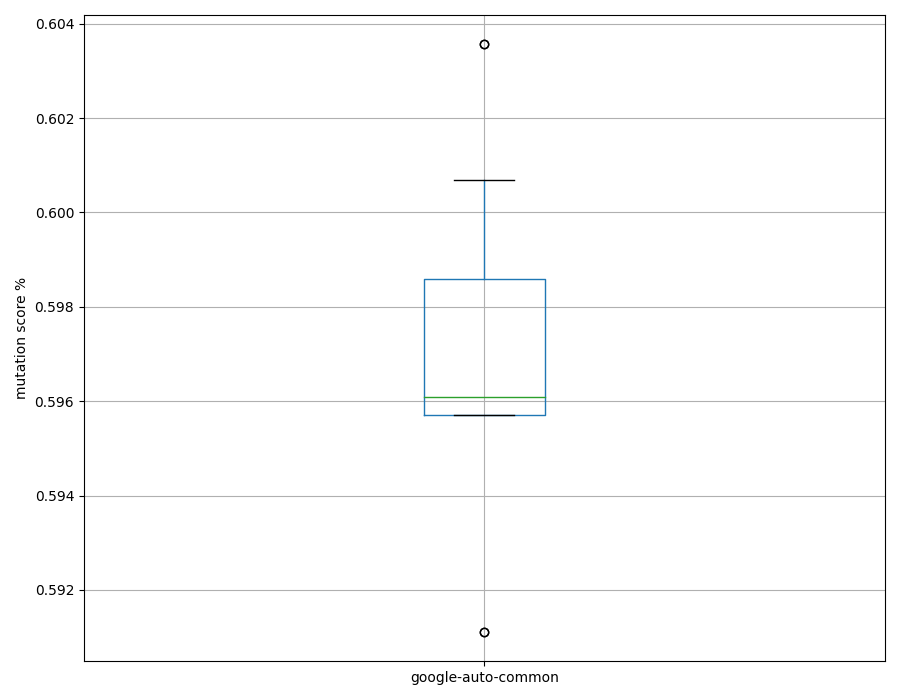
\includegraphics[scale=0.3]{images/full_75/boxplot_google-auto-common.png}}}
\end{figure}

\begin{figure}[h]
    \centering
    \subfloat{{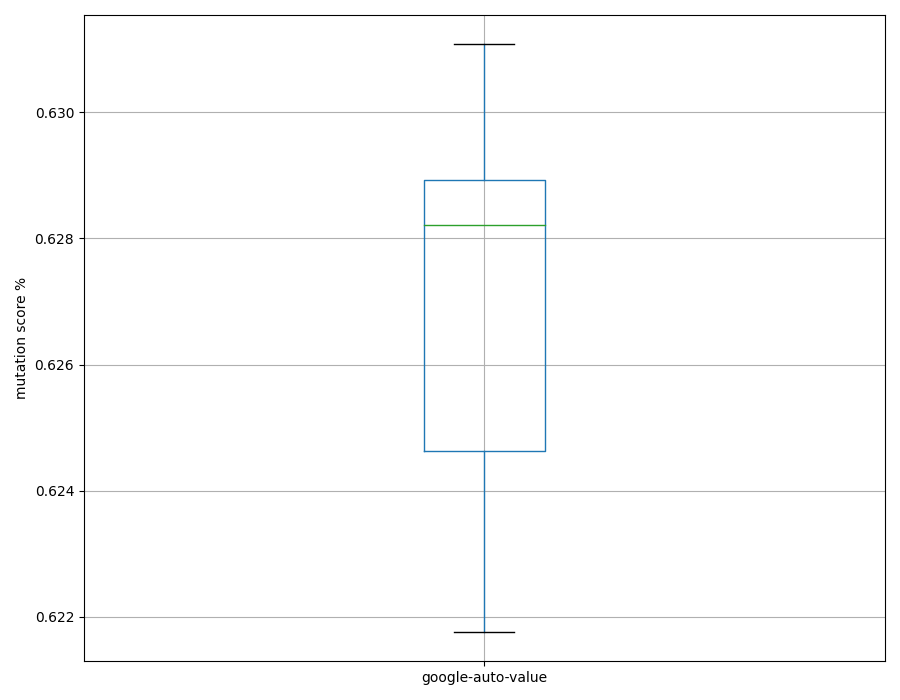
\includegraphics[scale=0.3]{images/full_75/boxplot_google-auto-value.png}}}
    \qquad
    \subfloat{{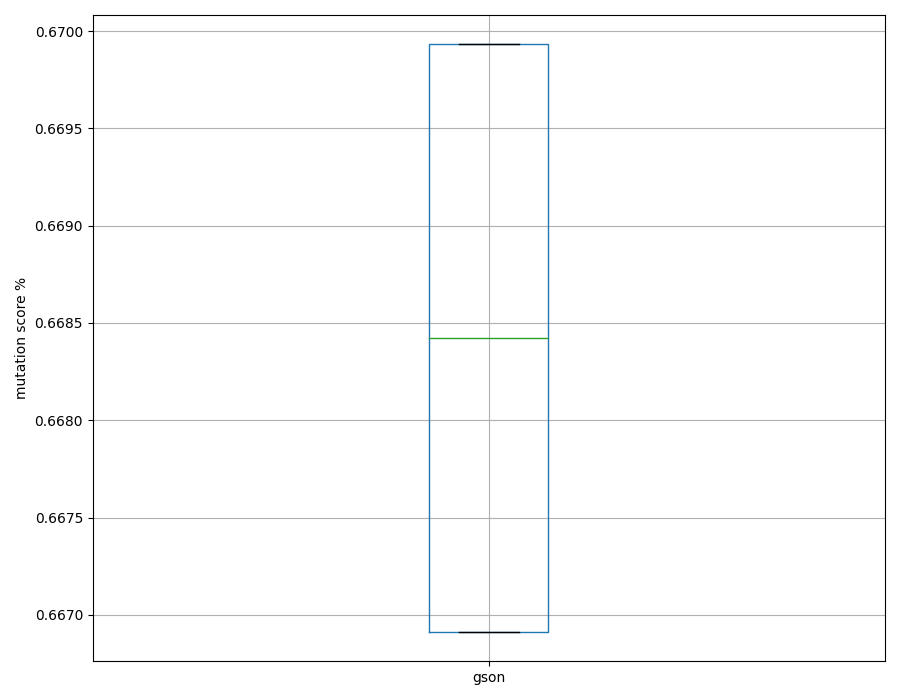
\includegraphics[scale=0.3]{images/full_75/boxplot_gson.png}}}
\end{figure}

\begin{figure}[h]
    \centering
    \subfloat{{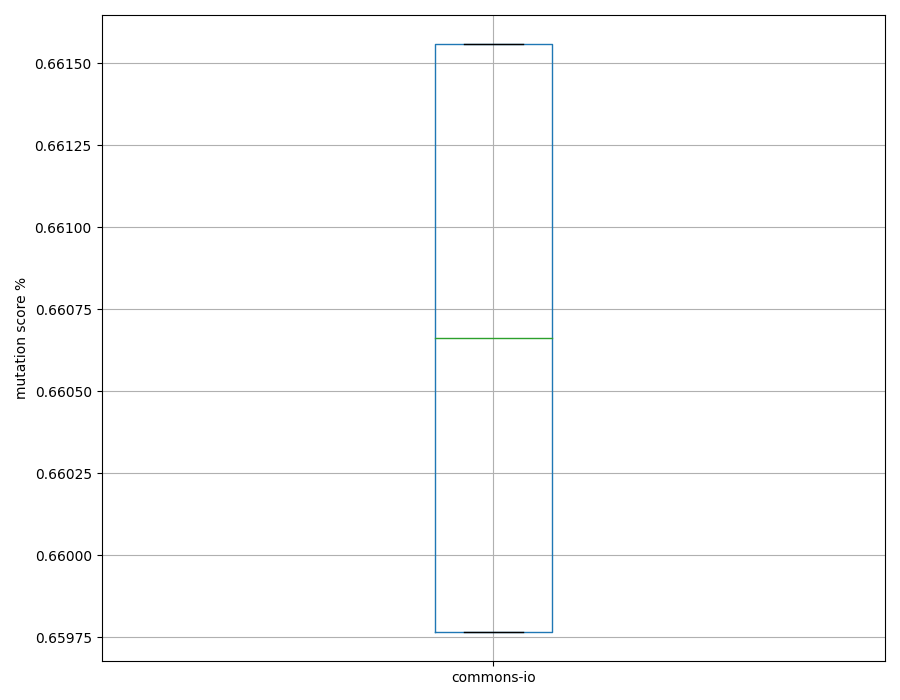
\includegraphics[scale=0.3]{images/full_75/boxplot_commons-io.png}}}
    \qquad
    \subfloat{{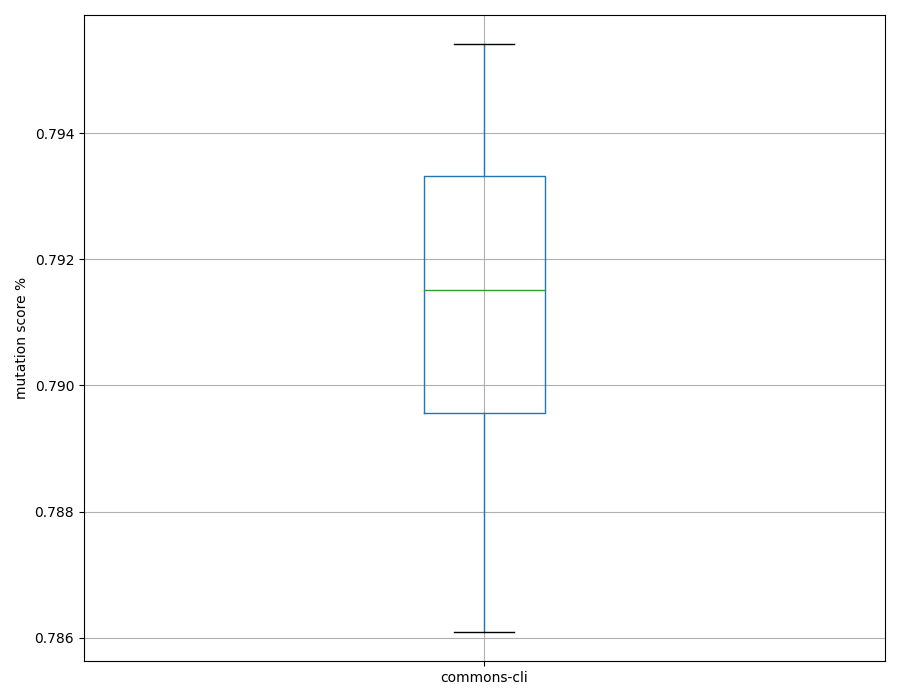
\includegraphics[scale=0.3]{images/full_75/boxplot_commons-cli.png}}}
\end{figure}

\begin{figure}[h]
    \centering
    \subfloat{{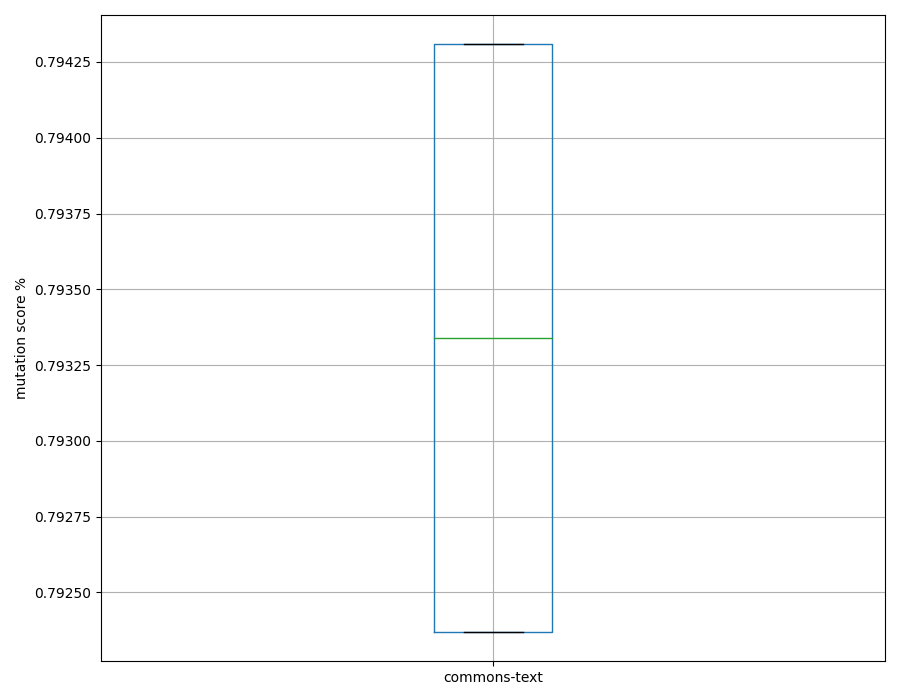
\includegraphics[scale=0.3]{images/full_75/boxplot_commons-text.png}}}
    \qquad
    \subfloat{{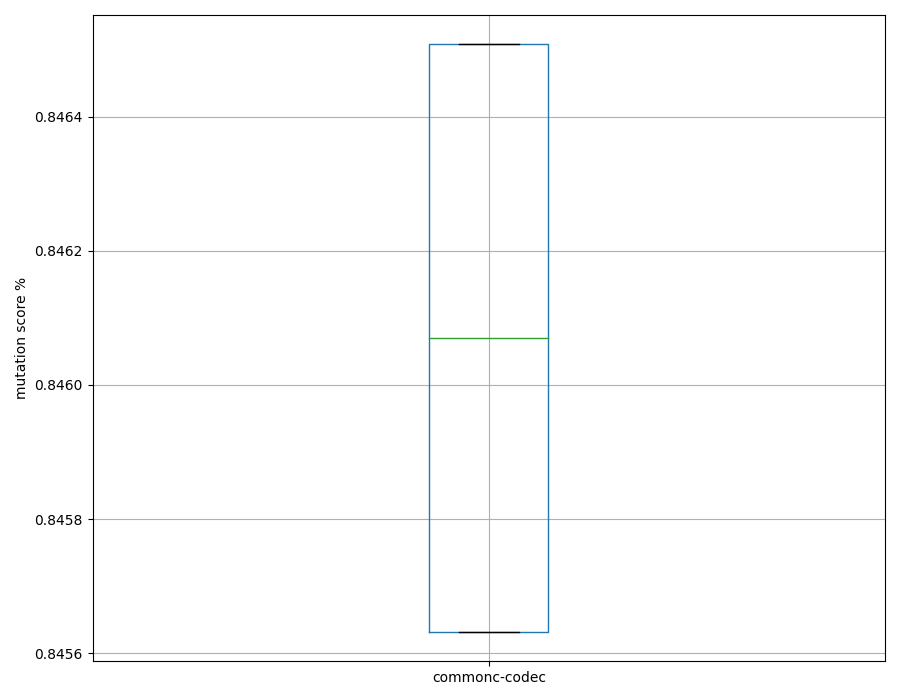
\includegraphics[scale=0.3]{images/full_75/boxplot_commonc-codec.png}}}
\end{figure}

\begin{figure}[h]
\centering
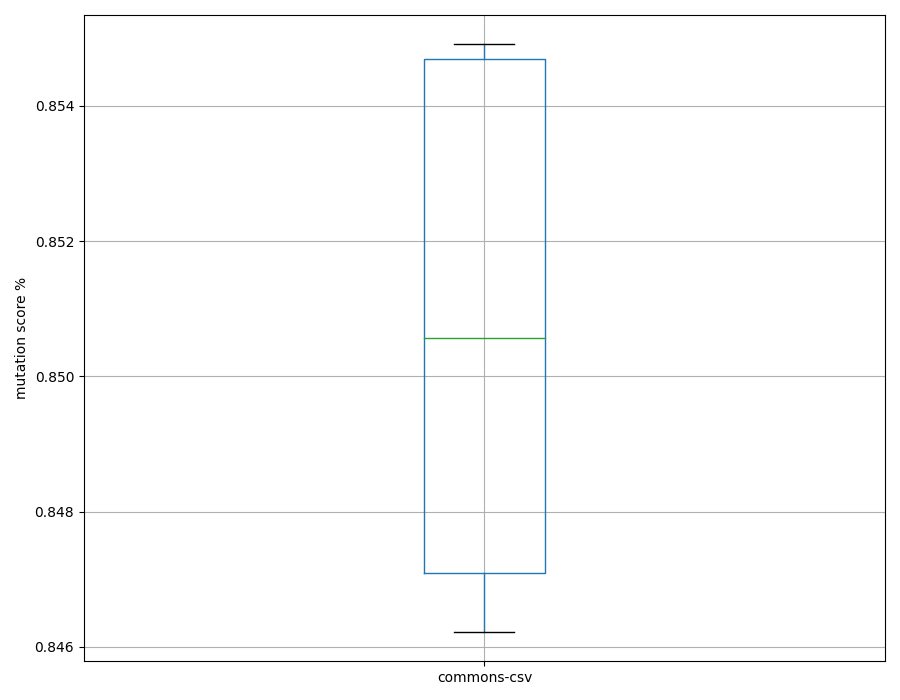
\includegraphics[scale=0.3]{images/full_75/boxplot_commons-csv.png}
\end{figure}


\chapter{Box-plots of samples per project without Levenshtein distance characteristic n*0.25 reduction}
\label{ap:no_distance_25}
\begin{figure}[h]
    \centering
    \subfloat{{\includegraphics[scale=0.32]{images/no_distance_25/boxplot_google-auto-service.png}}}
    \qquad
    \subfloat{{\includegraphics[scale=0.32]{images/no_distance_25/boxplot_scribejava-core.png}}}
\end{figure}

\begin{figure}[h]
    \centering
    \subfloat{{\includegraphics[scale=0.3]{images/no_distance_25/boxplot_google-auto-factory.png}}}
    \qquad
    \subfloat{{\includegraphics[scale=0.3]{images/no_distance_25/boxplot_google-auto-common.png}}}
\end{figure}

\begin{figure}[h]
    \centering
    \subfloat{{\includegraphics[scale=0.3]{images/no_distance_25/boxplot_google-auto-value.png}}}
    \qquad
    \subfloat{{\includegraphics[scale=0.3]{images/no_distance_25/boxplot_gson.png}}}
\end{figure}

\begin{figure}[h]
    \centering
    \subfloat{{\includegraphics[scale=0.3]{images/no_distance_25/boxplot_commons-io.png}}}
    \qquad
    \subfloat{{\includegraphics[scale=0.3]{images/no_distance_25/boxplot_commons-cli.png}}}
\end{figure}

\begin{figure}[h]
    \centering
    \subfloat{{\includegraphics[scale=0.3]{images/no_distance_25/boxplot_commons-text.png}}}
    \qquad
    \subfloat{{\includegraphics[scale=0.3]{images/no_distance_25/boxplot_commonc-codec.png}}}
\end{figure}

\begin{figure}[h]
\centering
\includegraphics[scale=0.3]{images/no_distance_25/boxplot_commons-csv.png}
\end{figure}

\chapter{Box-plots of samples per project without Levenshtein distance characteristic n*0.50 reduction}
\label{ap:no_distance_50}
\begin{figure}[h]
    \centering
    \subfloat{{\includegraphics[scale=0.32]{images/no_distance_50/boxplot_google-auto-service.png}}}
    \qquad
    \subfloat{{\includegraphics[scale=0.32]{images/no_distance_50/boxplot_scribejava-core.png}}}
\end{figure}

\begin{figure}[h]
    \centering
    \subfloat{{\includegraphics[scale=0.3]{images/no_distance_50/boxplot_google-auto-factory.png}}}
    \qquad
    \subfloat{{\includegraphics[scale=0.3]{images/no_distance_50/boxplot_google-auto-common.png}}}
\end{figure}

\begin{figure}[h]
    \centering
    \subfloat{{\includegraphics[scale=0.3]{images/no_distance_50/boxplot_google-auto-value.png}}}
    \qquad
    \subfloat{{\includegraphics[scale=0.3]{images/no_distance_50/boxplot_gson.png}}}
\end{figure}

\begin{figure}[h]
    \centering
    \subfloat{{\includegraphics[scale=0.3]{images/no_distance_50/boxplot_commons-io.png}}}
    \qquad
    \subfloat{{\includegraphics[scale=0.3]{images/no_distance_50/boxplot_commons-cli.png}}}
\end{figure}

\begin{figure}[h]
    \centering
    \subfloat{{\includegraphics[scale=0.3]{images/no_distance_50/boxplot_commons-text.png}}}
    \qquad
    \subfloat{{\includegraphics[scale=0.3]{images/no_distance_50/boxplot_commonc-codec.png}}}
\end{figure}

\begin{figure}[h]
\centering
\includegraphics[scale=0.3]{images/no_distance_50/boxplot_commons-csv.png}
\end{figure}

\chapter{Box-plots of samples per project without Levenshtein distance characteristic n*0.75 reduction}
\label{ap:no_distance_75}
\begin{figure}[h]
    \centering
    \subfloat{{\includegraphics[scale=0.32]{images/no_distance_75/boxplot_google-auto-service.png}}}
    \qquad
    \subfloat{{\includegraphics[scale=0.32]{images/no_distance_75/boxplot_scribejava-core.png}}}
\end{figure}

\begin{figure}[h]
    \centering
    \subfloat{{\includegraphics[scale=0.3]{images/no_distance_75/boxplot_google-auto-factory.png}}}
    \qquad
    \subfloat{{\includegraphics[scale=0.3]{images/no_distance_75/boxplot_google-auto-common.png}}}
\end{figure}

\begin{figure}[h]
    \centering
    \subfloat{{\includegraphics[scale=0.3]{images/no_distance_75/boxplot_google-auto-value.png}}}
    \qquad
    \subfloat{{\includegraphics[scale=0.3]{images/no_distance_75/boxplot_gson.png}}}
\end{figure}

\begin{figure}[h]
    \centering
    \subfloat{{\includegraphics[scale=0.3]{images/no_distance_75/boxplot_commons-io.png}}}
    \qquad
    \subfloat{{\includegraphics[scale=0.3]{images/no_distance_75/boxplot_commons-cli.png}}}
\end{figure}

\begin{figure}[h]
    \centering
    \subfloat{{\includegraphics[scale=0.3]{images/no_distance_75/boxplot_commons-text.png}}}
    \qquad
    \subfloat{{\includegraphics[scale=0.3]{images/no_distance_75/boxplot_commonc-codec.png}}}
\end{figure}

\begin{figure}[h]
\centering
\includegraphics[scale=0.3]{images/no_distance_75/boxplot_commons-csv.png}
\end{figure}







	
\end{appendices}

%comment out in the final version
%\listoftodos[Notes]

\end{document}